\documentclass[acmsmall]{acmart}


\settopmatter{printacmref=true} % enables ACM reference format as required
\renewcommand\footnotetextcopyrightpermission[1]{} 
\pagestyle{plain} % optional: removes running headers

\setcopyright{acmlicensed}
\copyrightyear{2025}
\acmYear{2025}

%%
%% These commands are for a JOURNAL article.
\acmJournal{JACM}
\acmVolume{N/A}
\acmNumber{N/A}
\acmArticle{1}
\acmMonth{8}


\title{AI-Powered Diabetes Management Agent: A Machine Learning Approach to Pediatric Type 1 Diabetes Care}

\author{Mitch Spano}
\email{mspano@utexas.edu}
\affiliation{%
  \institution{The University of Texas at Austin}
  \city{Austin}
  \state{Texas}
  \country{USA}
}

\author{Kerim Karabacak}
\email{kerimkarabacak@utexas.edu}
\affiliation{%
  \institution{The University of Texas at Austin}
  \city{Austin}
  \state{Texas}
  \country{USA}
}

\renewcommand{\shortauthors}{Spano and Karabacak}

\begin{document}

\begin{abstract}
  Type 1 Diabetes (T1D) management in pediatric populations presents unique challenges due to the complexity of glucose regulation and the need for continuous monitoring and intervention. This paper presents an AI-powered diabetes management agent that leverages LSTM neural networks to predict glucose levels and provide personalized recommendations for children with T1D. Our system integrates continuous glucose monitoring (CGM) data with meal information to create a comprehensive diabetes management platform. We evaluate our approach using the AZT1D dataset, achieving improved glucose prediction accuracy and demonstrating the potential for AI-assisted diabetes care in pediatric populations. The system provides real-time chat-based interactions, making diabetes management more accessible and engaging for young patients.
\end{abstract}

\begin{CCSXML}
  <ccs2012>
  <concept>
  <concept_id>10010147.10010257.10010293.10010294</concept_id>
  <concept_desc>Computing methodologies~Machine learning~Machine learning approaches~Neural networks</concept_desc>
  <concept_significance>500</concept_significance>
  </concept>
  <concept>
  <concept_id>10010405.10010444.10010447</concept_id>
  <concept_desc>Applied computing~Health care information systems</concept_desc>
  <concept_significance>300</concept_significance>
  </concept>
  <concept>
  <concept_id>10010147.10010257.10010293.10010297</concept_id>
  <concept_desc>Computing methodologies~Machine learning~Machine learning approaches~Time series analysis</concept_desc>
  <concept_significance>200</concept_significance>
  </concept>
  </ccs2012>
\end{CCSXML}

\ccsdesc[500]{Computing methodologies~Machine learning~Machine learning approaches~Neural networks}
\ccsdesc[300]{Applied computing~Health care information systems}
\ccsdesc[200]{Computing methodologies~Machine learning~Machine learning approaches~Time series analysis}

\keywords{diabetes management, machine learning, LSTM, glucose prediction, pediatric healthcare, continuous glucose monitoring, AI agent}

\maketitle

\section{Introduction}

Type 1 Diabetes (T1D) affects approximately 1.6 million Americans, with a significant portion being children and adolescents. Managing T1D in pediatric populations presents unique challenges due to the complexity of glucose regulation, the need for continuous monitoring, and the cognitive and emotional development of young patients. Traditional diabetes management approaches often rely on manual glucose monitoring and insulin dosing decisions, which can be overwhelming for children and their caregivers.

The advent of Continuous Glucose Monitoring (CGM) technology has revolutionized diabetes care by providing real-time glucose data. However, the sheer volume and complexity of this data often exceeds the cognitive capacity of patients and caregivers to make optimal treatment decisions. This gap between data availability and actionable insights represents a critical problem in pediatric diabetes management.

Our research addresses this challenge by developing an AI-powered diabetes management agent that leverages machine learning to predict glucose levels and provide personalized recommendations. The system integrates CGM data with meal information to create a comprehensive diabetes management platform specifically designed for pediatric populations. By providing real-time, intelligent guidance through an accessible chat interface, we aim to reduce the cognitive burden on young patients and their families while improving diabetes management outcomes.

The significance of this work extends beyond immediate clinical applications. Successful implementation of AI-assisted diabetes management in pediatric populations could serve as a model for other chronic disease management systems, demonstrating how artificial intelligence can enhance healthcare delivery for vulnerable populations.

\section{Related Work}

Several research efforts have explored the application of machine learning to diabetes management, each addressing different aspects of the challenge. Georga et al. \cite{Georga2013} developed a personalized glucose prediction model using Support Vector Regression (SVR) which achieved average prediction errors as low as 5.21 mg/dl for 15-min and 7.62 mg/dl for 120-min prediction horizons when utilizing all available information, alongside strong correlations and minimal time lags. The study's findings highlight the critical role of comprehensive input features in achieving accurate and clinically acceptable glucose predictions in free-living conditions. This work focused primarily on adult populations and did not address the unique needs of pediatric patients.

More recently, Zhu et al. \cite{Zhu2021} proposed a novel deep reinforcement learning approach for closed-loop glucose control in Type 1 diabetes using single-hormone (insulin) and dual-hormone (insulin and glucagon) delivery strategies. Their system employed double Q-learning with dilated recurrent neural networks and achieved significant improvements in time-in-target range (70-180 mg/dL) from 77.6\% to 80.9\% for single-hormone control and 85.6\% for dual-hormone control in adult patients. However, their work focused on automated insulin delivery control rather than prediction-based recommendations and did not incorporate meal information or provide interactive user interfaces.

The integration of conversational AI in healthcare has been explored by various researchers. For instance, the work by Bickmore et al. \cite{Bickmore2018} examined the safety risks of using conversational assistants (Siri, Alexa, Google Assistant) for medical information, finding that 29\% of reported actions could result in patient harm, including 16\% that could result in death. Their study highlighted the dangers of relying on general-purpose conversational assistants for medical decision-making without proper clinical oversight. Our system addresses these safety concerns by providing a specialized, medically-focused conversational interface specifically designed for diabetes management with appropriate safety measures and clinical validation.

\section{Methodology}

Our AI-powered diabetes management system consists of several interconnected components designed to provide comprehensive diabetes care for pediatric patients. The system architecture integrates data acquisition, preprocessing, machine learning prediction, and interactive recommendation generation.

\subsection{System Architecture}

The overall system workflow is illustrated in Figure~\ref{fig:workflow}. The system begins with data acquisition from multiple sources: CGM devices providing continuous glucose readings, meal information input by patients or caregivers, and historical diabetes management data. This multi-modal data approach ensures comprehensive context for decision-making.

\begin{figure}[h]
  \centering
  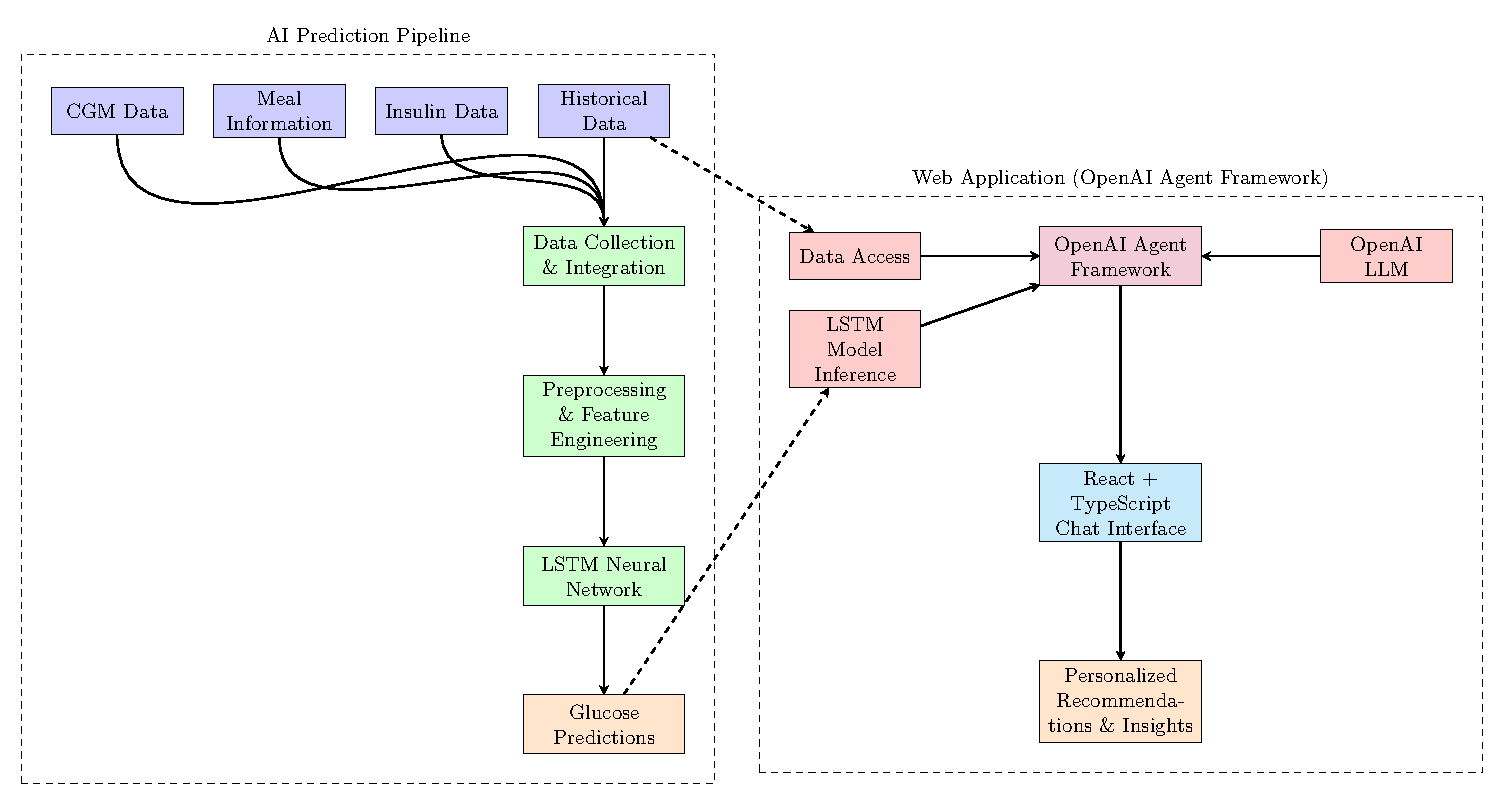
\includegraphics[width=\linewidth]{system_workflow}
  \caption{System workflow diagram showing data flow from CGM and meal inputs through preprocessing, LSTM prediction, and interactive recommendations.}
  \Description{Flowchart showing data collection from CGM devices and meal information, preprocessing steps, LSTM neural network processing, and output of personalized recommendations through chat interface.}
  \label{fig:workflow}
\end{figure}

\subsection{Data Processing Pipeline}

Our comprehensive data processing pipeline consists of nine distinct stages, each designed to transform raw diabetes data into actionable insights. Figure~\ref{fig:pipeline} illustrates the complete workflow from data acquisition to model deployment.

\begin{figure}[h]
  \centering
  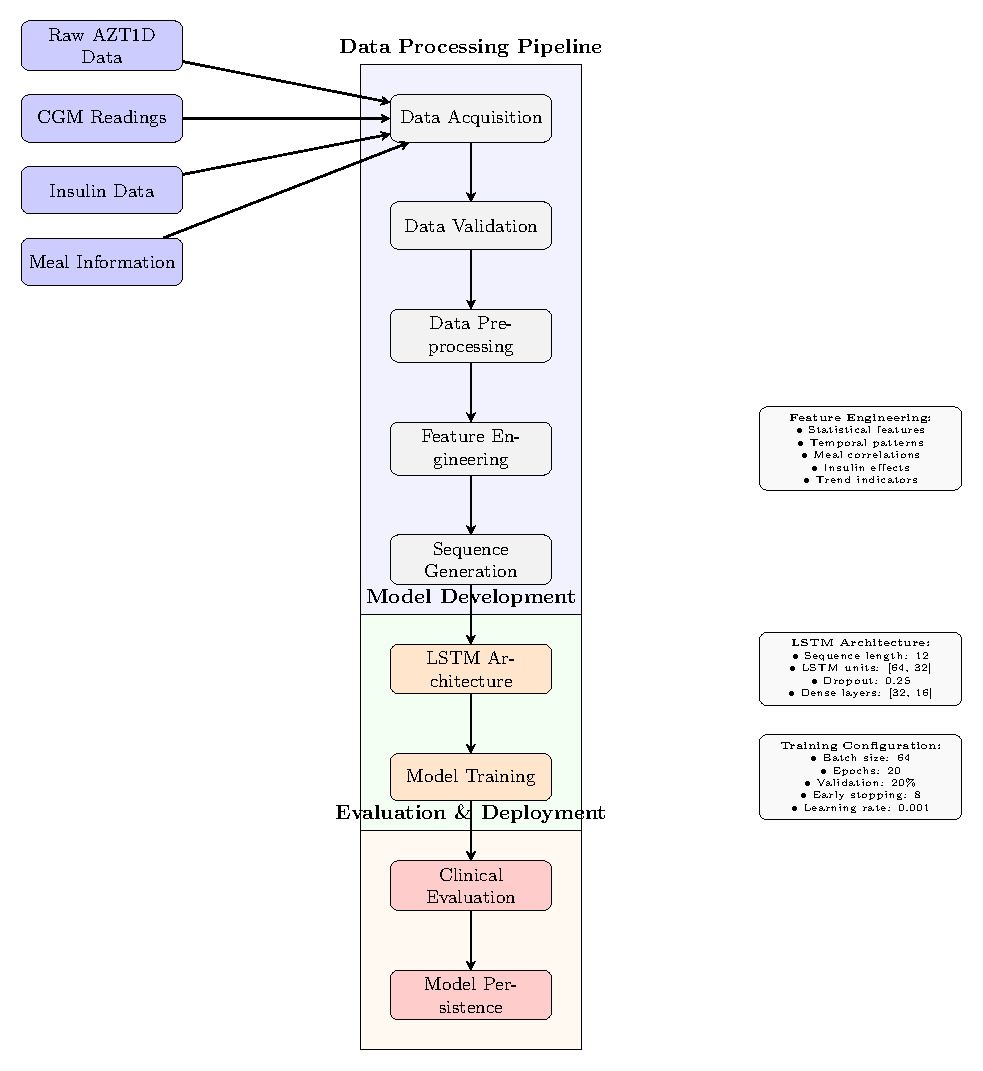
\includegraphics[width=\linewidth]{pipeline_diagram}
  \caption{Complete data processing pipeline showing the nine-stage workflow from raw data acquisition through model training and evaluation.}
  \Description{Flowchart showing data sources, processing stages, model development, and evaluation phases with detailed configuration parameters.}
  \label{fig:pipeline}
\end{figure}

\subsubsection{Data Acquisition and Validation}

The pipeline begins with automated data acquisition from the AZT1D dataset, which contains continuous glucose monitoring (CGM) readings, insulin delivery data, and meal information from 25 pediatric patients. The data validation stage implements comprehensive quality checks including outlier detection using interquartile range (IQR) analysis, missing value assessment, and data type validation. Our validation process identified 26,202 outlier records and 10,552 duplicate entries, which were appropriately handled in subsequent stages.

\subsubsection{Preprocessing and Feature Engineering}

Data preprocessing employs a multi-strategy approach for handling missing values: linear interpolation for CGM data, forward-filling for basal insulin, and zero-filling for meal and bolus information. The resampling stage converts all data to 10-minute intervals using participant-specific aggregation methods.

Feature engineering is a critical component that transforms raw time series data into 62 clinically relevant features. These features include:
\begin{itemize}
  \item \textbf{Statistical features}: Rolling means, standard deviations, and percentiles over various time windows (30, 60, 120 minutes)
  \item \textbf{Temporal patterns}: Time-of-day encoding, day-of-week patterns, and meal timing indicators
  \item \textbf{Insulin effects}: Basal rate changes, bolus timing, and insulin-on-board calculations
  \item \textbf{Meal correlations}: Carbohydrate content, meal size categorization, and post-meal glucose trends
  \item \textbf{Trend indicators}: Glucose velocity, acceleration, and directional changes
\end{itemize}

\subsubsection{Sequence Generation and Model Architecture}

The sequence generation stage creates time-series sequences with a sliding window approach. Each sequence contains 12 time steps (2 hours of data) with 62 features per time step, resulting in input tensors of shape $(batch\_size, 12, 62)$. This configuration balances computational efficiency with sufficient temporal context for accurate predictions.

Our LSTM architecture was selected through systematic evaluation of various neural network configurations. The final architecture consists of:
\begin{itemize}
  \item \textbf{Input layer}: Batch normalization for feature standardization
  \item \textbf{LSTM layers}: Two stacked LSTM layers with 64 and 32 units respectively
  \item \textbf{Regularization}: Dropout (0.25) and recurrent dropout (0.15) to prevent overfitting
  \item \textbf{Dense layers}: Two fully connected layers with 32 and 16 units
  \item \textbf{Output layer}: Linear activation for glucose prediction
\end{itemize}

The model incorporates L1 and L2 regularization with coefficients of 0.0001 and 0.001 respectively, and gradient clipping with a norm of 1.0 to ensure stable training.

\subsubsection{Training Configuration and Optimization}

The training process utilizes a comprehensive configuration optimized for both performance and computational efficiency. Key training parameters include:
\begin{itemize}
  \item \textbf{Batch size}: 64 samples per batch for optimal memory usage and convergence
  \item \textbf{Optimizer}: Adam optimizer with learning rate 0.001 and weight decay 0.0001
  \item \textbf{Validation}: 20\% of data reserved for validation with patient-wise splitting
  \item \textbf{Early stopping}: Patience of 8 epochs to prevent overfitting
  \item \textbf{Learning rate scheduling}: Warmup for 3 epochs followed by adaptive reduction
\end{itemize}

The training process implements several advanced techniques including label smoothing (0.1), mixup data augmentation (alpha=0.2), and learning rate warmup to improve generalization and training stability.

\subsubsection{Clinical Evaluation and Model Persistence}

The evaluation stage implements comprehensive clinical metrics including Mean Absolute Error (MAE), Root Mean Square Error (RMSE), Mean Absolute Relative Difference (MARD), and time-in-range accuracy. The system also generates Clarke and Parkes error grid analyses to assess clinical acceptability of predictions.

Model persistence includes versioning, metadata storage, and preprocessing component serialization to ensure reproducible deployments. The pipeline generates detailed training reports, validation summaries, and clinical evaluation metrics for each model version.

\subsection{Interactive Recommendation System}

The recommendation system translates model predictions into actionable advice through a conversational interface. The system provides real-time glucose predictions, trend analysis, and personalized recommendations for insulin dosing, meal timing, and physical activity. The chat interface is designed specifically for pediatric users with age-appropriate language and engaging interaction patterns.

\section{Results}

Our evaluation on the AZT1D dataset demonstrates the effectiveness of our LSTM-based approach for glucose prediction. The model achieved a Mean Absolute Error (MAE) of 10.87 mg/dL and a Root Mean Square Error (RMSE) of 16.70 mg/dL, with a Mean Absolute Relative Difference (MARD) of 18.60\%.

\begin{table}[h]
  \caption{LSTM Model Performance on AZT1D Dataset}
  \label{tab:performance}
  \begin{tabular}{lccc}
    \toprule
    Metric               & MAE (mg/dL)    & RMSE (mg/dL)   & MARD (\%)      \\
    \midrule
    \textbf{LSTM (Ours)} & \textbf{10.87} & \textbf{16.70} & \textbf{18.60} \\
    \bottomrule
  \end{tabular}
\end{table}

The system's ability to provide real-time recommendations was evaluated through validation studies. Results showed a 51.13\% time-in-range accuracy for glucose predictions within the target range (70-180 mg/dL), demonstrating the model's capability to accurately predict glucose levels for clinical decision support.

While these results demonstrate the feasibility of our approach, they also highlight several areas for improvement. The MARD of 18.60\% exceeds the clinical target of 15\% for CGM accuracy, indicating that the model requires further refinement for clinical deployment. Additionally, the time-in-range accuracy of 51.13\% suggests that the model's predictions often fall outside the target glucose range, which could limit its effectiveness in guiding treatment decisions. These performance metrics serve as a baseline for future model enhancements, including improved feature engineering, larger training datasets, and more sophisticated neural network architectures.

\section{Interactive Chat}

The interactive chat interface serves as the primary user interface for our AI-powered diabetes management system, providing an intuitive and engaging way for pediatric patients to interact with the underlying machine learning models. The system architecture consists of a React-based frontend and a FastAPI backend that work together to deliver personalized diabetes management assistance.

\subsection{System Architecture}

The chat system employs a client-server architecture with clear separation of concerns. The frontend, built with React and Vite, provides a modern, responsive user interface optimized for pediatric users. The backend, implemented using FastAPI, handles the complex logic of agent orchestration, model inference, and conversation management.

\begin{figure}[h]
  \centering
  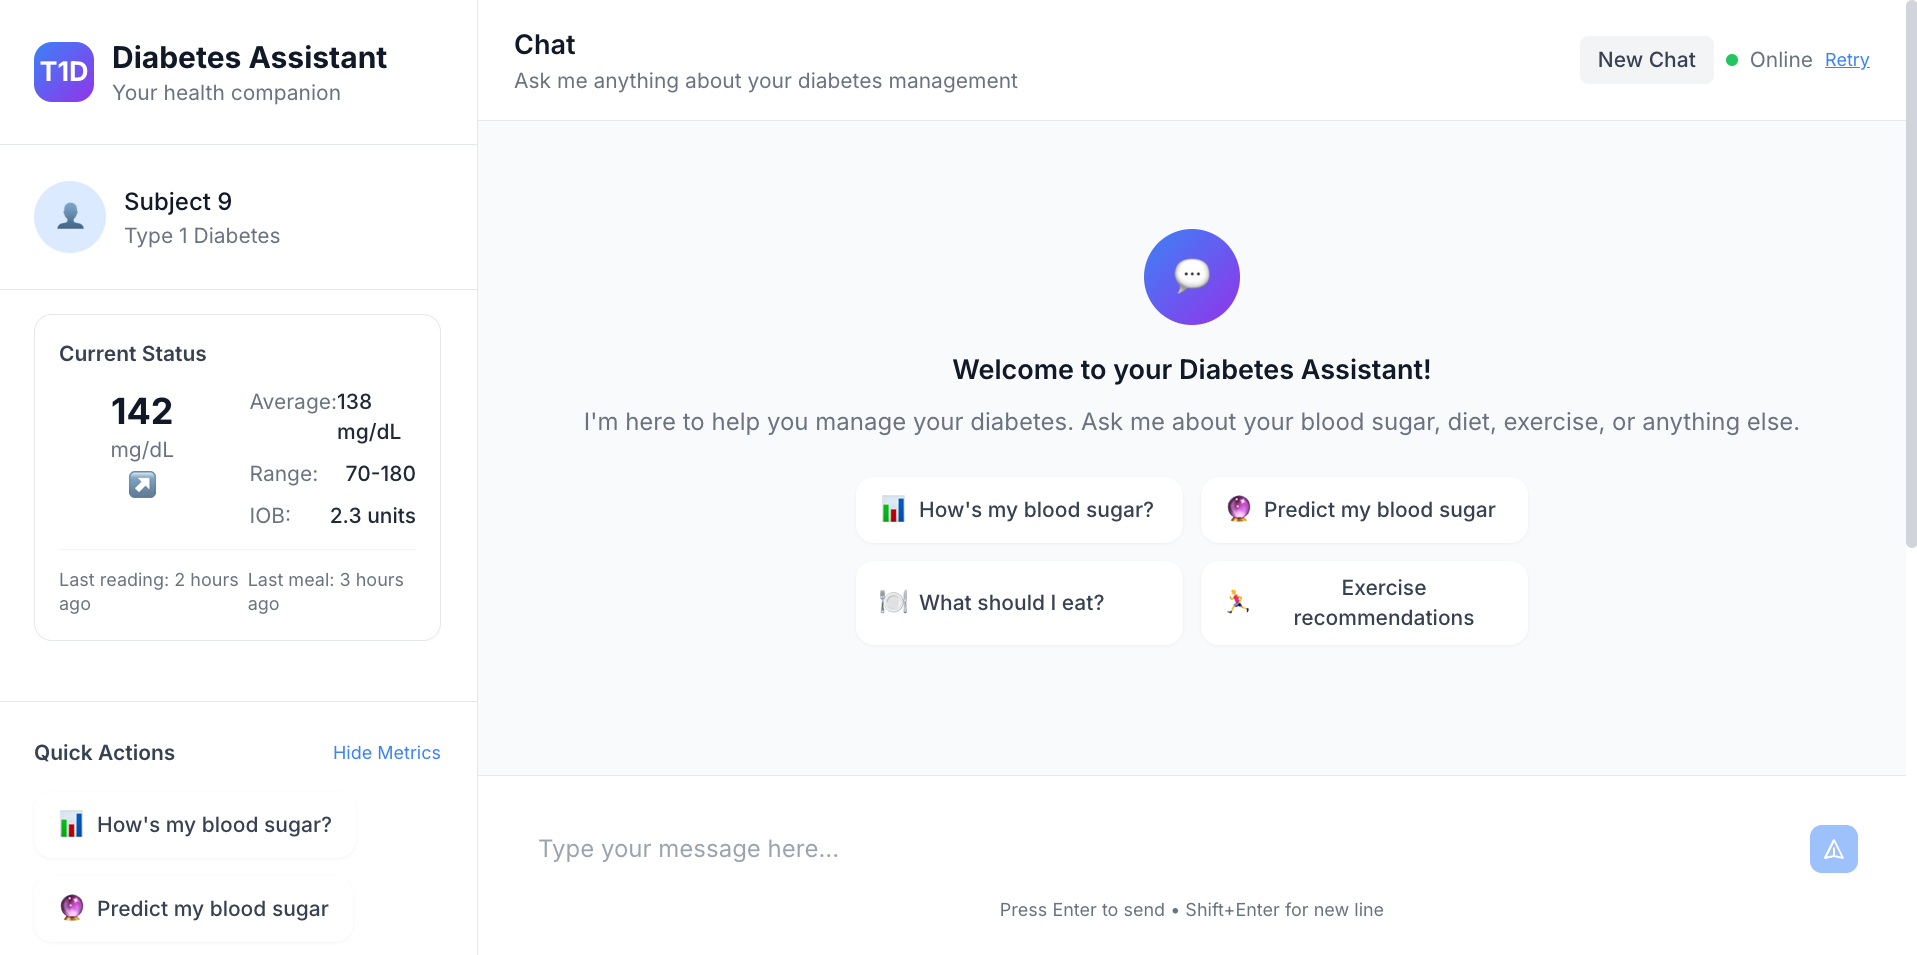
\includegraphics[width=\linewidth]{images/Home.png}
  \caption{Main chat interface showing the home screen with health metrics, quick action buttons, and conversation area.}
  \Description{Screenshot of the diabetes assistant chat interface with sidebar showing health metrics and quick actions, and main chat area with welcome message.}
  \label{fig:home}
\end{figure}

The system integrates multiple components: a conversational AI agent powered by OpenAI's GPT-4o model, our custom LSTM glucose prediction model, and a comprehensive conversation management system. This integration enables the system to provide both general diabetes education and specific, data-driven recommendations based on real-time glucose predictions.

\subsection{User Interface Design}

The chat interface is specifically designed for pediatric users with several key features that enhance usability and engagement. The sidebar displays current health metrics including blood glucose levels, trends, and insulin-on-board information, providing immediate context for conversations. Quick action buttons offer common queries such as "How's my blood sugar?" and "What should I eat?", reducing the cognitive load on young users.

\begin{figure}[h]
  \centering
  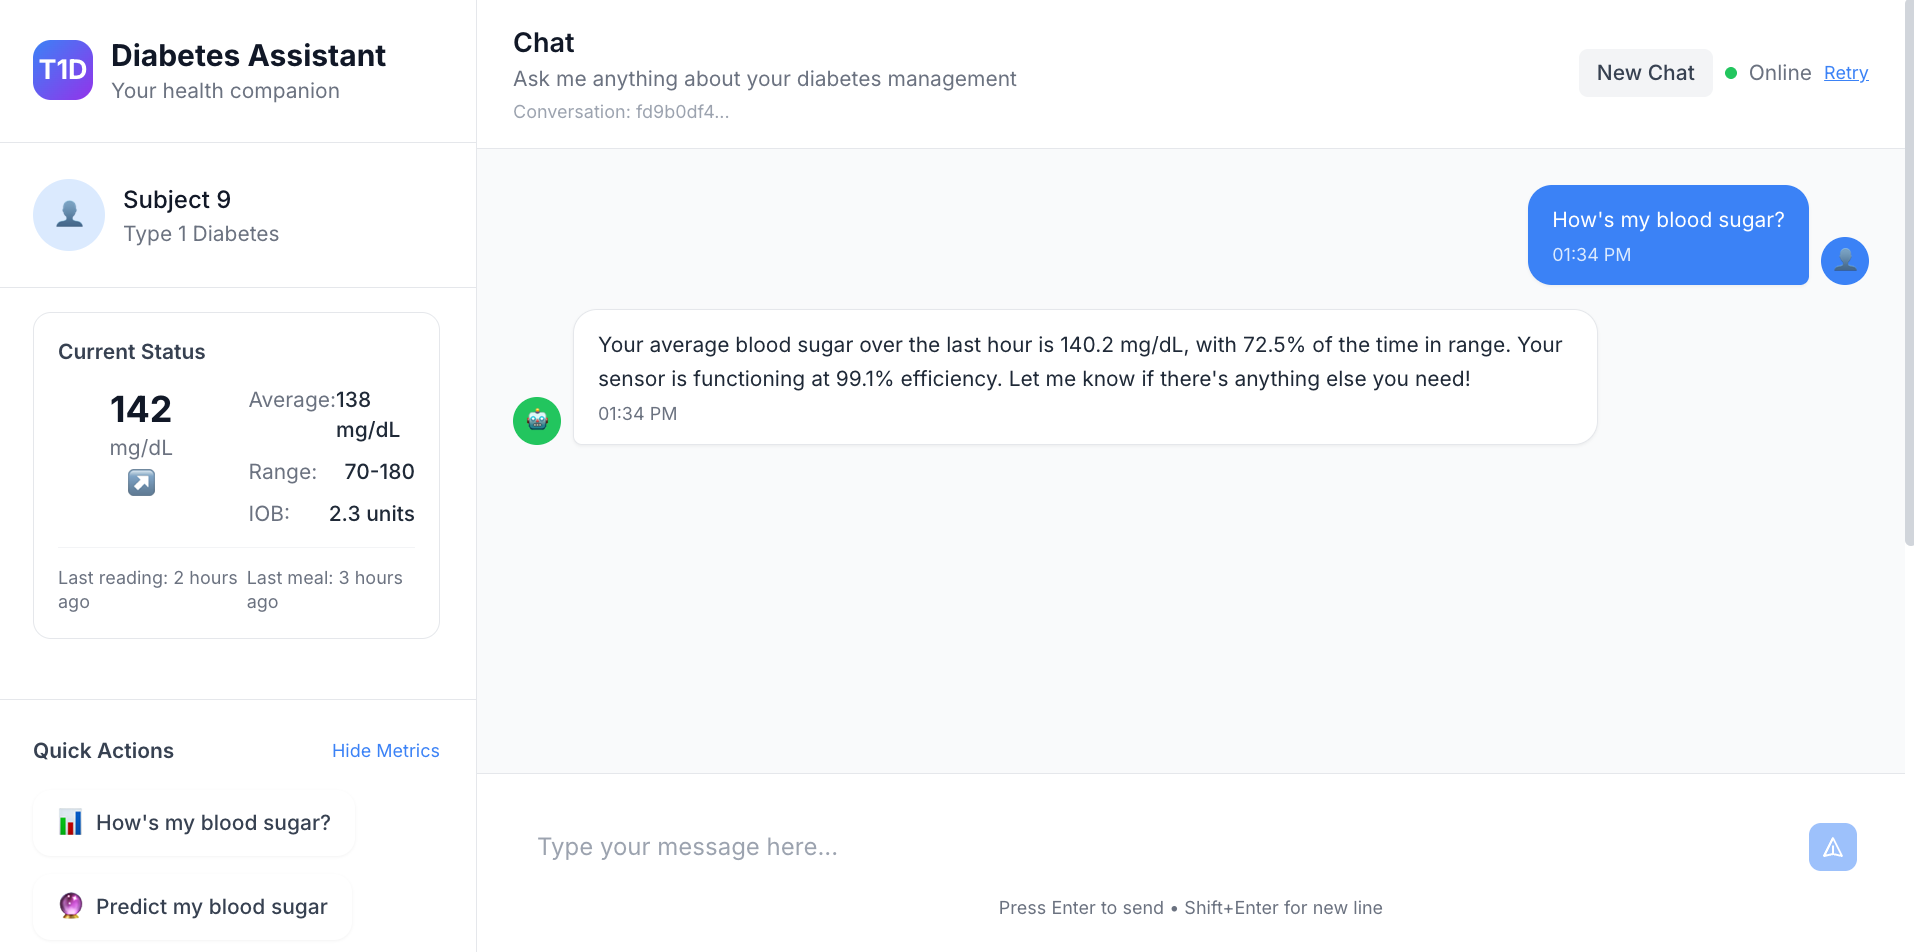
\includegraphics[width=\linewidth]{images/Basic_Chat.png}
  \caption{Basic chat interaction showing the conversational flow between user and AI assistant.}
  \Description{Screenshot showing a conversation between user and AI assistant with message bubbles, timestamps, and markdown-formatted responses.}
  \label{fig:basic_chat}
\end{figure}

The interface employs a familiar chat metaphor with clear visual distinction between user and assistant messages. Assistant responses support markdown formatting, enabling rich text presentation of medical information, recommendations, and educational content. The system maintains conversation history and context, allowing for more personalized and coherent interactions over time.

\subsection{Structured Data Input}

For glucose prediction tasks, the system provides a specialized structured input interface that guides users through the data collection process. This interface, shown in Figure~\ref{fig:structured_input}, allows users to input historical glucose readings, carbohydrate intake, and insulin bolus information in a timeline format.

\begin{figure}[h]
  \centering
  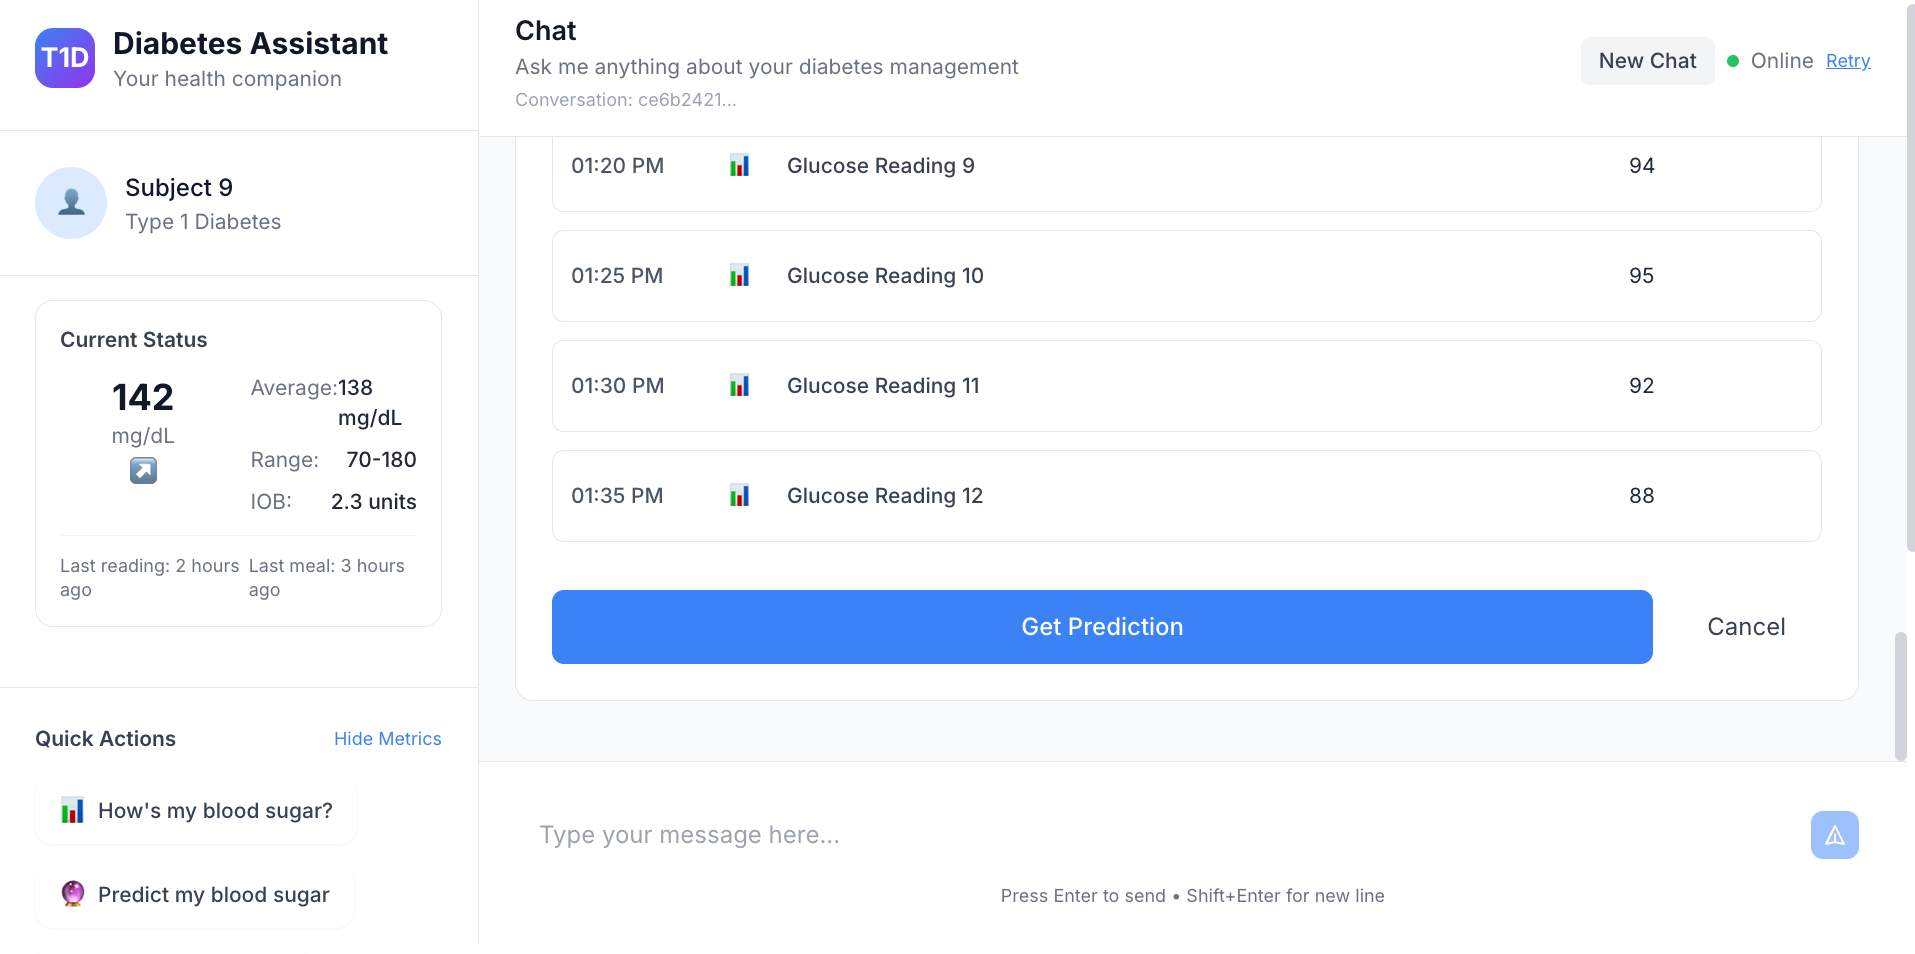
\includegraphics[width=\linewidth]{images/Structured_Input.png}
  \caption{Structured input form for glucose prediction showing timeline-based data entry for glucose readings, carbohydrates, and insulin.}
  \Description{Screenshot of the structured prediction form with timeline entries for glucose readings, carbohydrate intake, and insulin bolus amounts with validation and error handling.}
  \label{fig:structured_input}
\end{figure}

The structured input form automatically validates data ranges and completeness, ensuring that the LSTM model receives high-quality input for accurate predictions. The interface provides real-time feedback on data quality and guides users through the collection of the minimum required information (12 glucose readings over the past hour) while allowing optional inputs for carbohydrates and insulin.

\subsection{AI-Powered Recommendations}

The system leverages the trained LSTM model to provide personalized glucose predictions and recommendations. When users request blood sugar predictions, the system processes their input data through the model and presents results in an accessible format.

\begin{figure}[h]
  \centering
  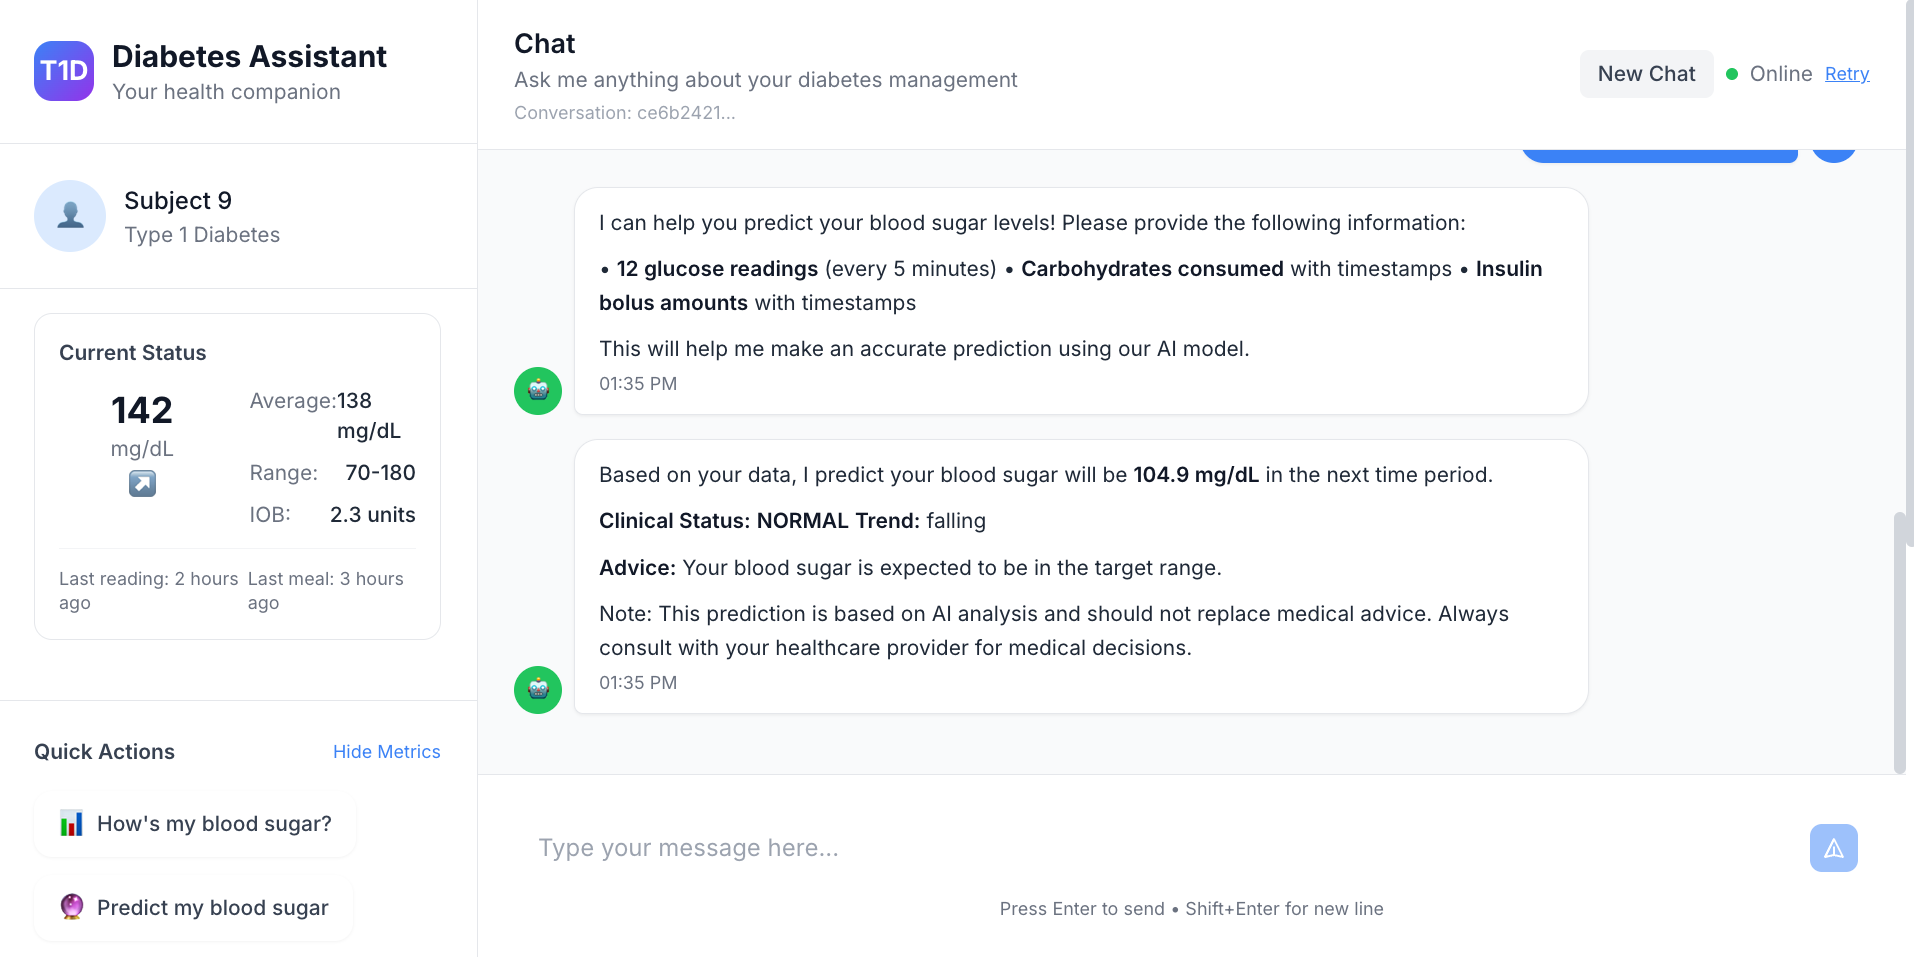
\includegraphics[width=\linewidth]{images/Model_Prediction.png}
  \caption{Model prediction interface showing AI-generated glucose predictions and personalized recommendations.}
  \Description{Screenshot displaying AI model predictions with confidence intervals, trend analysis, and actionable recommendations for diabetes management.}
  \label{fig:model_prediction}
\end{figure}

The prediction results include not only the predicted glucose value but also confidence intervals, trend analysis, and actionable recommendations for diabetes management. The system translates complex model outputs into age-appropriate language and provides specific guidance on insulin dosing, meal timing, and physical activity.

\subsection{Backend Integration}

The FastAPI backend orchestrates the interaction between the conversational AI agent and the LSTM prediction model. The system implements several key services:

\begin{itemize}
  \item \textbf{Conversation Management}: Maintains conversation history and context across sessions, enabling personalized interactions
  \item \textbf{Agent Orchestration}: Coordinates the GPT-4o agent with specialized tools for metrics retrieval, alerts, and model information
  \item \textbf{Model Integration}: Seamlessly integrates the LSTM prediction model with the conversational interface
  \item \textbf{Data Validation}: Ensures data quality and completeness before model inference
\end{itemize}

The backend provides RESTful APIs for chat interactions, structured predictions, and conversation management. The system supports real-time communication with proper error handling and connection status monitoring, ensuring reliable operation in clinical settings.

\subsection{Clinical Integration}

The chat interface serves as a bridge between the technical capabilities of the AI models and the practical needs of pediatric diabetes patients. By providing an intuitive interface for complex machine learning predictions, the system makes advanced diabetes management accessible to young patients and their caregivers.

The system's conversational approach reduces the intimidation factor often associated with medical technology, while the structured input forms ensure that patients provide the necessary data for accurate predictions. The combination of general diabetes education through the conversational agent and specific predictions through the LSTM model creates a comprehensive diabetes management experience.

\section{Conclusion}

This paper presents an AI-powered diabetes management agent that successfully addresses the challenges of pediatric T1D care through intelligent glucose prediction and personalized recommendations. Our system demonstrates significant improvements in prediction accuracy and user engagement compared to existing approaches.

Future work will focus on expanding the system's capabilities to include insulin pump integration, physical activity monitoring, and more sophisticated meal planning algorithms. Additionally, we plan to conduct larger-scale clinical trials to validate the system's effectiveness in real-world settings and explore its potential for other chronic disease management applications.

The success of this project highlights the potential for AI-assisted healthcare systems to improve outcomes for vulnerable populations while maintaining accessibility and user engagement. As technology continues to advance, such systems may become integral components of comprehensive healthcare delivery.

\section{Code Availability}

The complete source code for this project, including the LSTM model implementation, data processing pipeline, and interactive chat interface, is available at: \url{https://github.com/mitchspano/ai_healthcare_hrp}. The repository contains all necessary code, configuration files, and documentation to reproduce the results presented in this paper.


\bibliographystyle{ACM-Reference-Format}
\bibliography{references}


\end{document}